\documentclass[a4paper, 12pt]{article}
\usepackage[margin=2cm]{geometry}
\usepackage{graphicx}
\usepackage{caption}

\graphicspath{{Images}}
\renewcommand{\familydefault}{\sfdefault}

\author{BE19B009 - Shobhan Karthick}
\title{Assignment 3 \\ Hopfield network}
\date{}

\begin{document}

\maketitle

\section{Data Visualization}
\label{visual}

The 3 files \textbf{ball.txt}, \textbf{cat.txt}, \textbf{mona.txt} were read using the \texttt{Pandas},a Python module and the data was stored in 2D-arrays and visualized in Figures \ref{fig:Q1_1}, \ref{fig:Q1_2}, \ref{fig:Q1_3} using the \texttt{matplotlib} module.
\\

\vspace{1 em}
\begin{center}
\begin{minipage}{0.45\linewidth}
    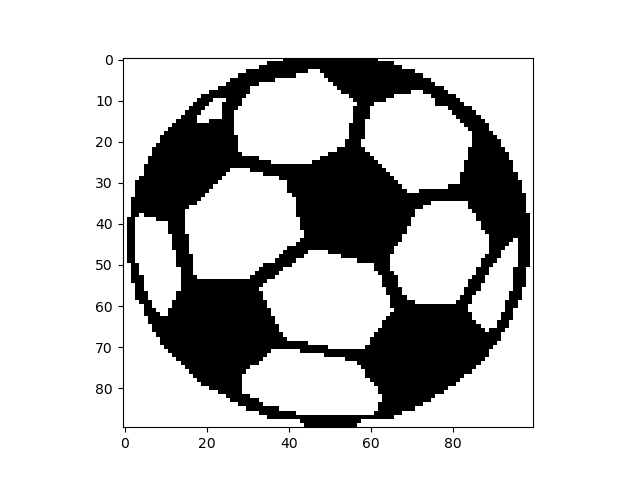
\includegraphics[width=\textwidth]{Q1_1}
    \captionof{figure}{Image visualization of the ball }
    \label{fig:Q1_1}
\end{minipage}
\hfill
\begin{minipage}{0.45\linewidth}
    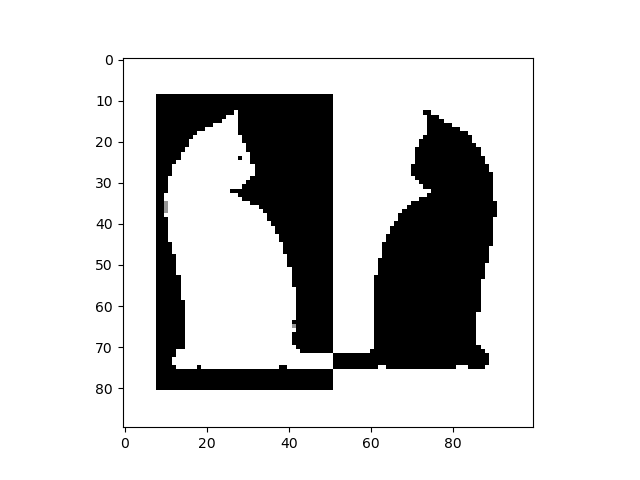
\includegraphics[width=\textwidth]{Q1_2}
    \captionof{figure}{Image visualization of the cat }
    \label{fig:Q1_2}
\end{minipage}
\vspace{1.5 em}

\begin{minipage}{0.45\linewidth}
    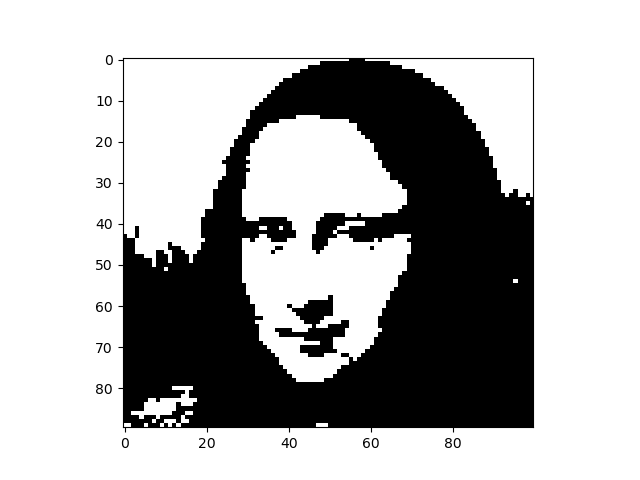
\includegraphics[width=\textwidth]{Q1_3}
    \captionof{figure}{Image visualization of the Mona Lisa }
    \label{fig:Q1_3}
\end{minipage}
\end{center}

\section{Input images}
\vspace{1 em}
\begin{center}
\begin{minipage}{0.45\linewidth}
    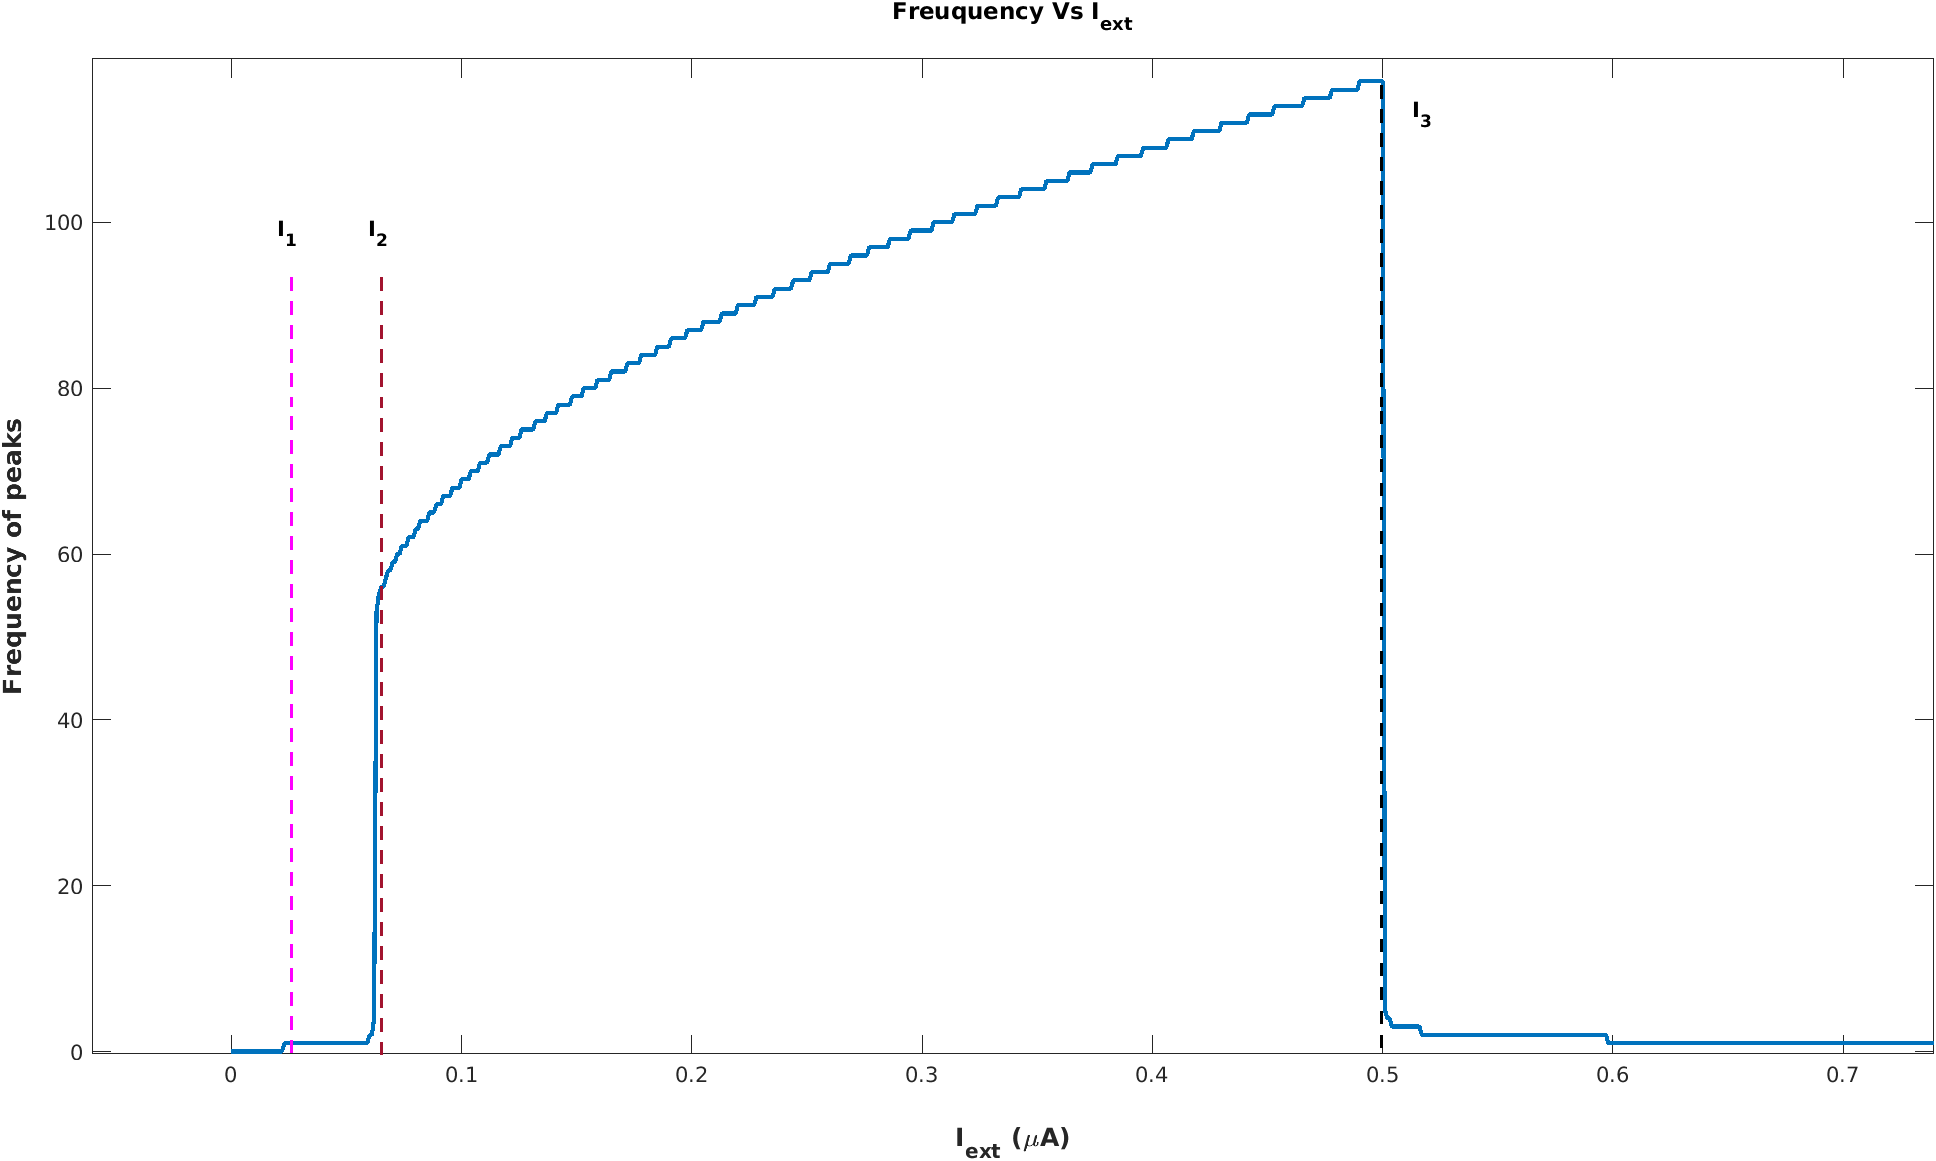
\includegraphics[width=\textwidth]{Q2_1}
    \captionof{figure}{Cut image of the ball }
    \label{fig:Q1_1}
\end{minipage}
\hfill
\begin{minipage}{0.45\linewidth}
    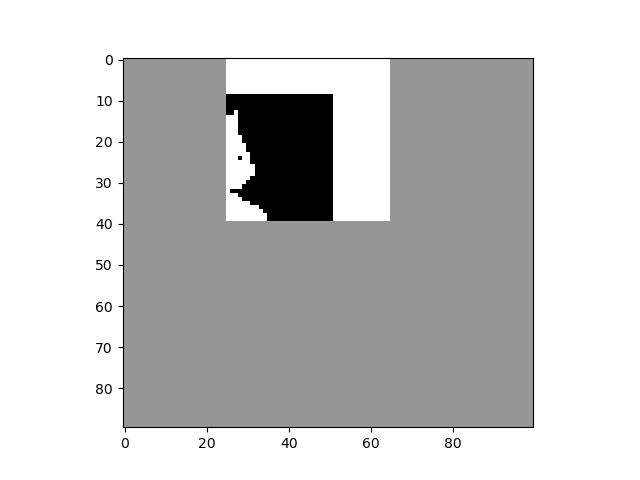
\includegraphics[width=\textwidth]{Q2_2}
    \captionof{figure}{Cut image of the cat }
    \label{fig:Q1_2}
\end{minipage}
\vspace{1.5 em}

\begin{minipage}{0.45\linewidth}
    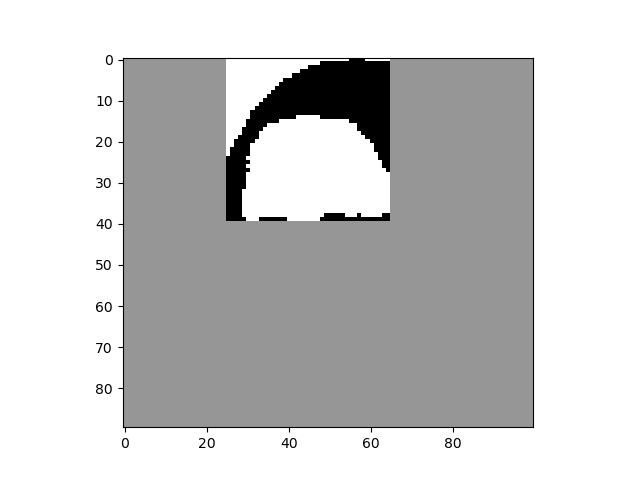
\includegraphics[width=\textwidth]{Q2_3}
    \captionof{figure}{Cut image of the Mona Lisa }
    \label{fig:Q1_3}
\end{minipage}
\end{center}



\section{0\% Weightage for Ball}

\subsection{Simulation}
\begin{center}
\begin{minipage}{0.45\linewidth}
    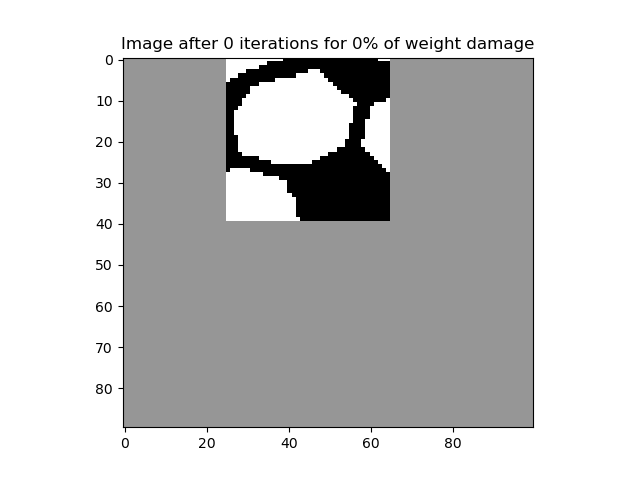
\includegraphics[width=\textwidth]{Q20}
    \captionof{figure}{At 0 iterations}
    \label{fig:Q1_1}
\end{minipage}
\hfill
\begin{minipage}{0.45\linewidth}
    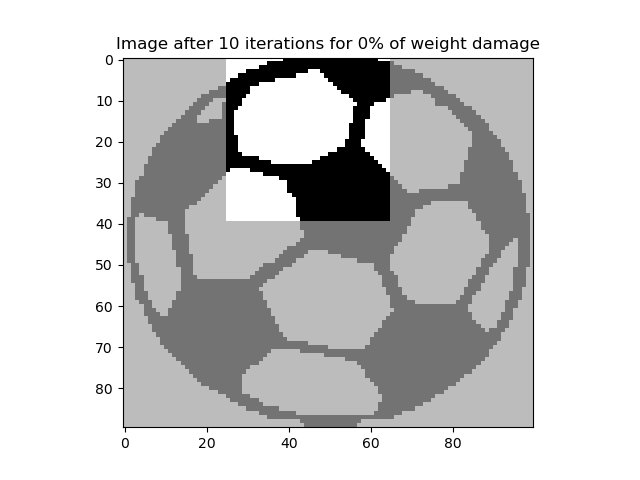
\includegraphics[width=\textwidth]{Q21}
    \captionof{figure}{At 10 iterations}
    \label{fig:Q1_2}
\end{minipage}
\vspace{1.5 em}

\begin{minipage}{0.45\linewidth}
    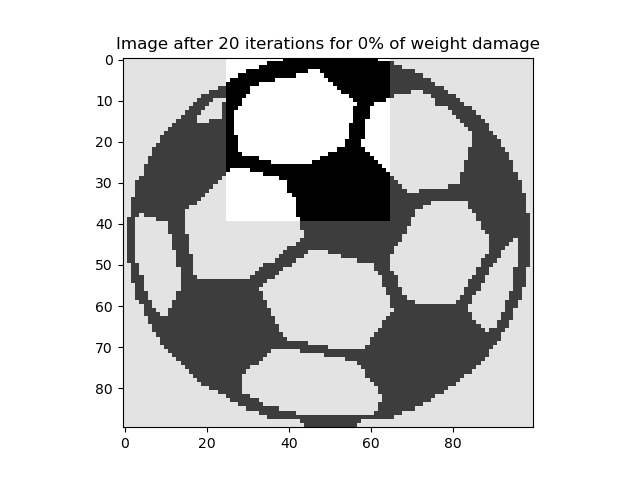
\includegraphics[width=\textwidth]{Q22}
    \captionof{figure}{At 20 iterations}
    \label{fig:Q1_1}
\end{minipage}
\hfill
\begin{minipage}{0.45\linewidth}
    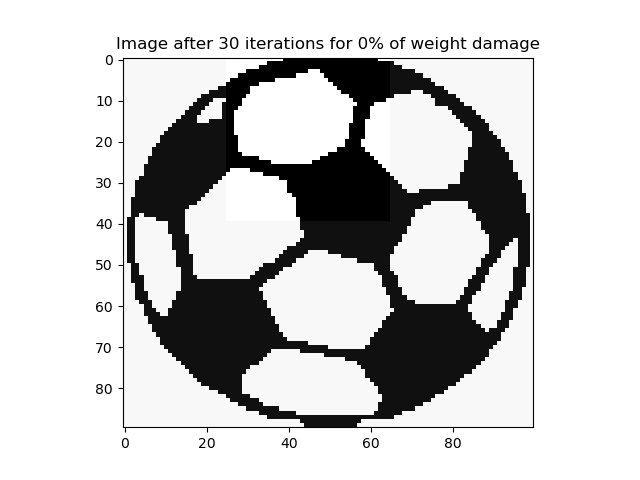
\includegraphics[width=\textwidth]{Q23}
    \captionof{figure}{At 30 iterations}
    \label{fig:Q1_2}
\end{minipage}
\vspace{1.5 em}


\begin{minipage}{0.45\linewidth}
    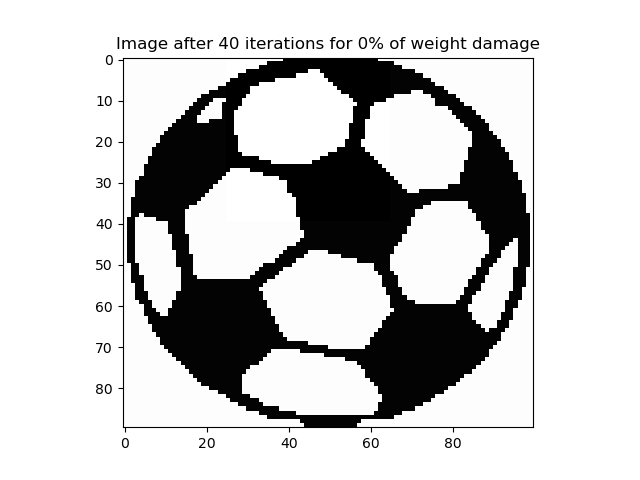
\includegraphics[width=\textwidth]{Q24}
    \captionof{figure}{At 40 iterations}
    \label{fig:Q1_3}
\end{minipage}
\end{center}

\subsection{Root mean squared error}

\begin{center}
\begin{minipage}{0.7\linewidth}
    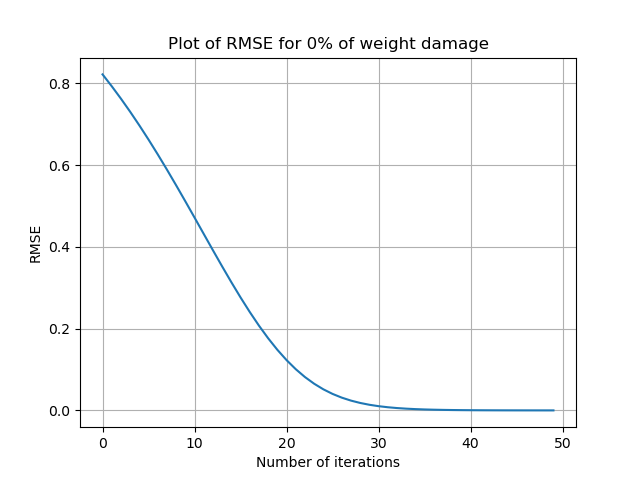
\includegraphics[width=\textwidth]{rmse4}
    \captionof{figure}{RMSE for 50 iteration at 0\% weightage}
    \label{fig:Q1_3}
\end{minipage}
\end{center}


\section{25\% Weightage for Ball}

\subsection{Simulation}
\begin{center}
\begin{minipage}{0.45\linewidth}
    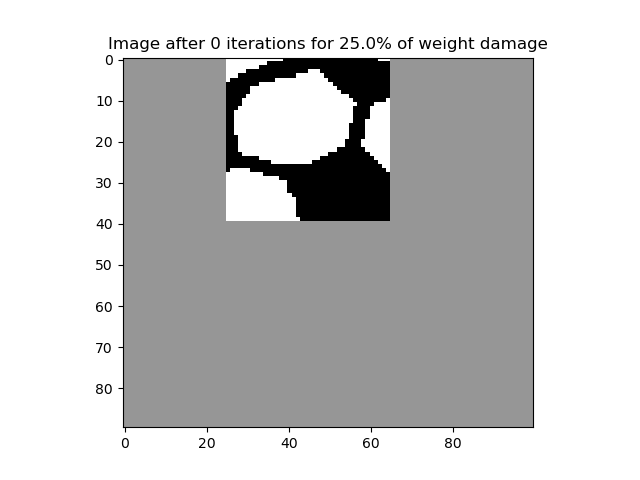
\includegraphics[width=\textwidth]{Q30}
    \captionof{figure}{At 0 iterations}
    \label{fig:Q1_1}
\end{minipage}
\hfill
\begin{minipage}{0.45\linewidth}
    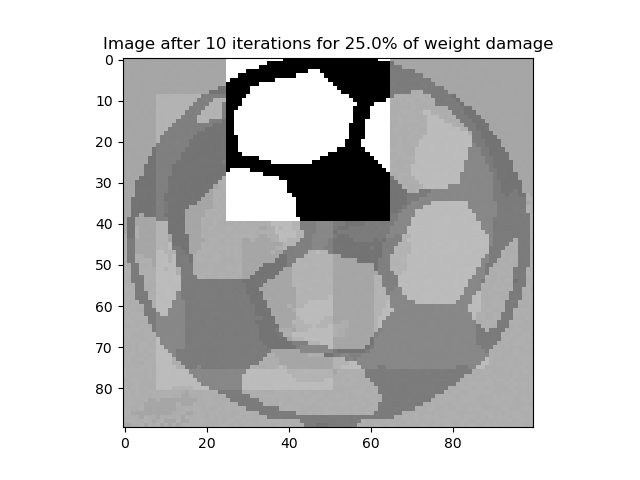
\includegraphics[width=\textwidth]{Q31}
    \captionof{figure}{At 10 iterations}
    \label{fig:Q1_2}
\end{minipage}
\vspace{1.5 em}

\begin{minipage}{0.45\linewidth}
    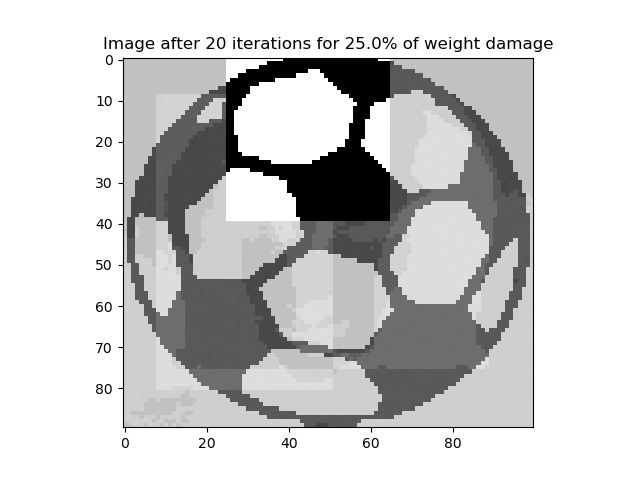
\includegraphics[width=\textwidth]{Q32}
    \captionof{figure}{At 20 iterations}
    \label{fig:Q1_1}
\end{minipage}
\hfill
\begin{minipage}{0.45\linewidth}
    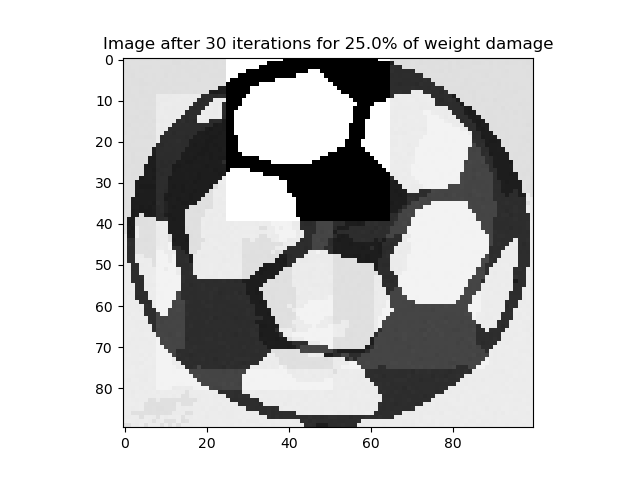
\includegraphics[width=\textwidth]{Q33}
    \captionof{figure}{At 30 iterations}
    \label{fig:Q1_2}
\end{minipage}
\vspace{1.5 em}

\begin{minipage}{0.45\linewidth}
    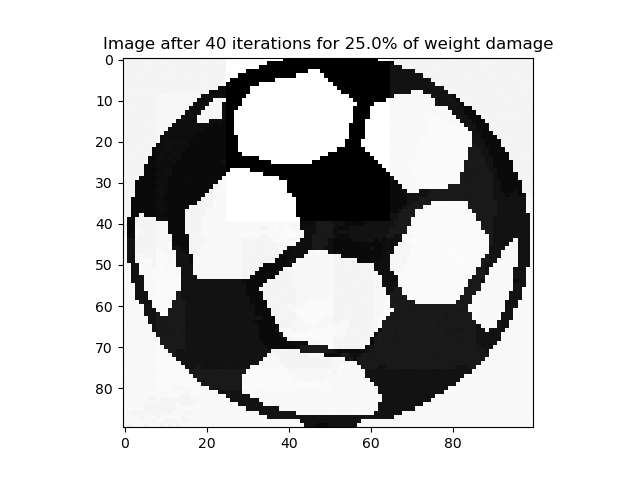
\includegraphics[width=\textwidth]{Q34}
    \captionof{figure}{At 40 iterations}
    \label{fig:Q1_1}
\end{minipage}
\hfill
\begin{minipage}{0.45\linewidth}
    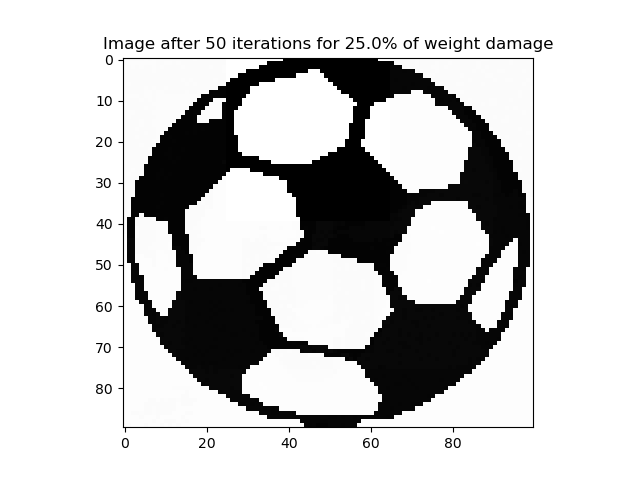
\includegraphics[width=\textwidth]{Q35}
    \captionof{figure}{At 50 iterations}
    \label{fig:Q1_2}
\end{minipage}
\vspace{1.5 em}

\begin{minipage}{0.45\linewidth}
    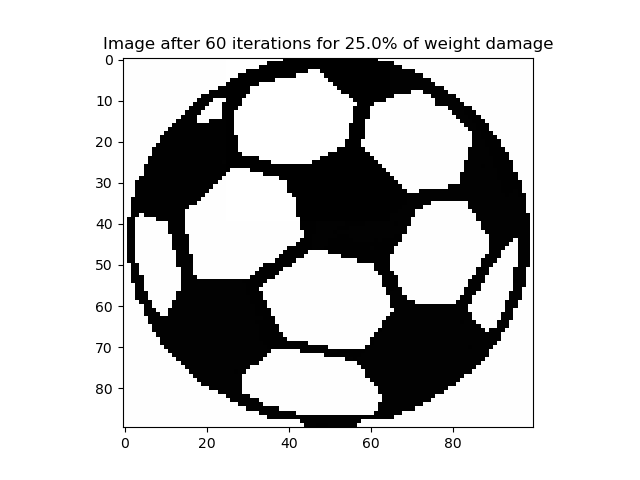
\includegraphics[width=\textwidth]{Q36}
    \captionof{figure}{At 60 iterations}
    \label{fig:Q1_1}
\end{minipage}
\hfill
\begin{minipage}{0.45\linewidth}
    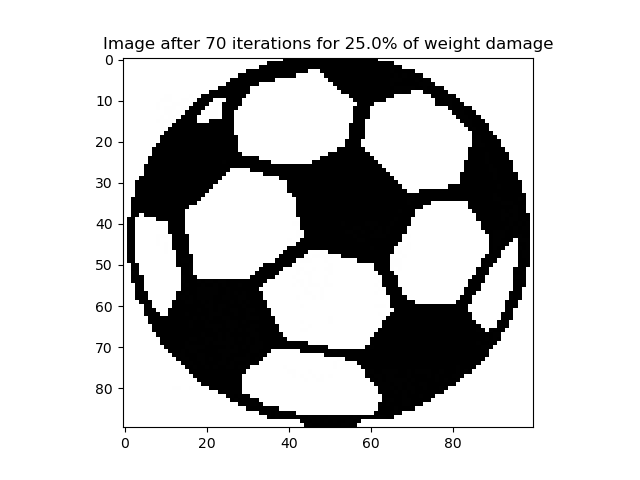
\includegraphics[width=\textwidth]{Q37}
    \captionof{figure}{At 70 iterations}
    \label{fig:Q1_2}
\end{minipage}
\vspace{1.5 em}

\begin{minipage}{0.45\linewidth}
    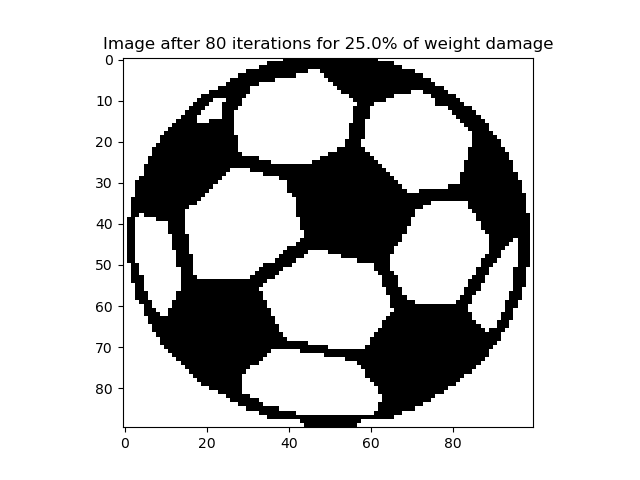
\includegraphics[width=\textwidth]{Q38}
    \captionof{figure}{At 80 iterations}
    \label{fig:Q1_1}
\end{minipage}
\hfill
\begin{minipage}{0.45\linewidth}
    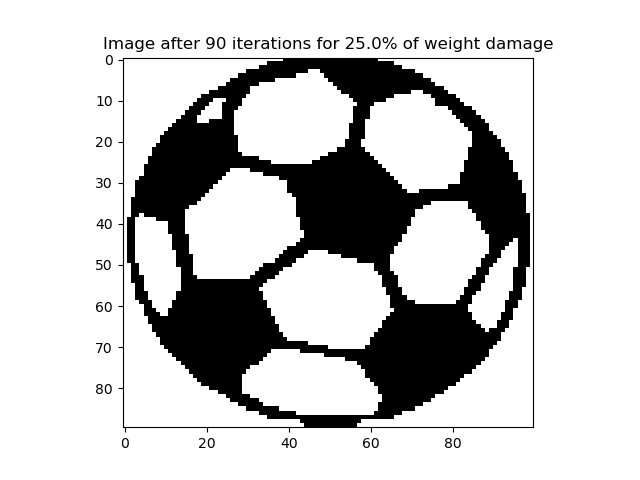
\includegraphics[width=\textwidth]{Q39}
    \captionof{figure}{At 90 iterations}
    \label{fig:Q1_2}
\end{minipage}
\vspace{1.5 em}
\end{center}

\subsection{Root mean squared error}

\begin{center}
\begin{minipage}{0.7\linewidth}
    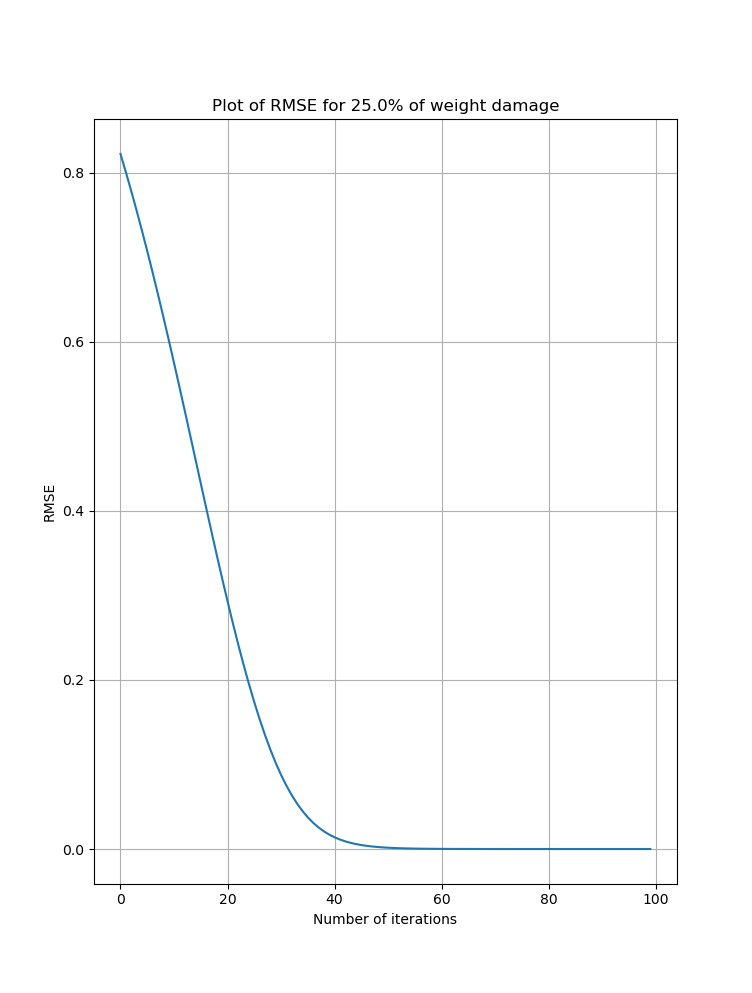
\includegraphics[width=\textwidth]{rmse_Q3}
    \captionof{figure}{RMSE for 100 iteration at 25\% weightage}
    \label{fig:Q1_3}
\end{minipage}
\end{center}


\section{50\% Weightage for Ball}

\subsection{Simulation}
\begin{center}
\begin{minipage}{0.45\linewidth}
    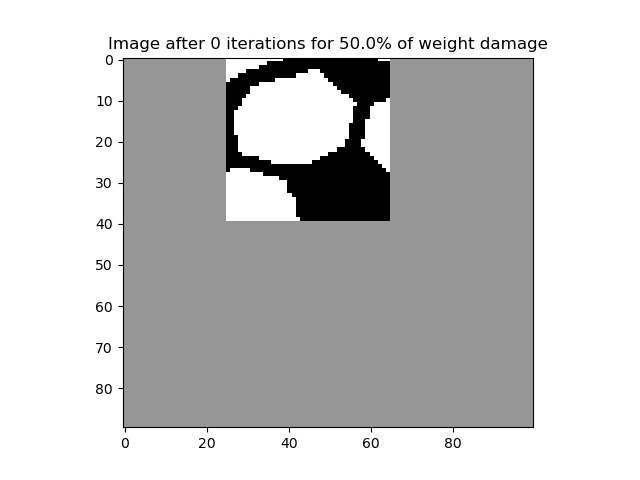
\includegraphics[width=\textwidth]{Q40}
    \captionof{figure}{At 0 iterations}
    \label{fig:Q1_1}
\end{minipage}
\hfill
\begin{minipage}{0.45\linewidth}
    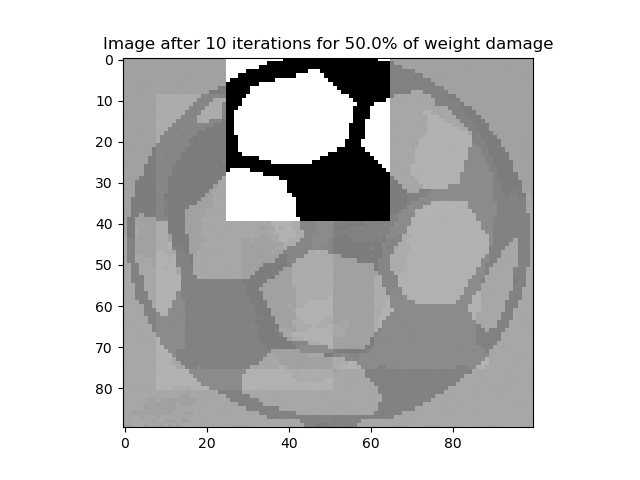
\includegraphics[width=\textwidth]{Q41}
    \captionof{figure}{At 10 iterations}
    \label{fig:Q1_2}
\end{minipage}
\vspace{1.5 em}

\begin{minipage}{0.45\linewidth}
    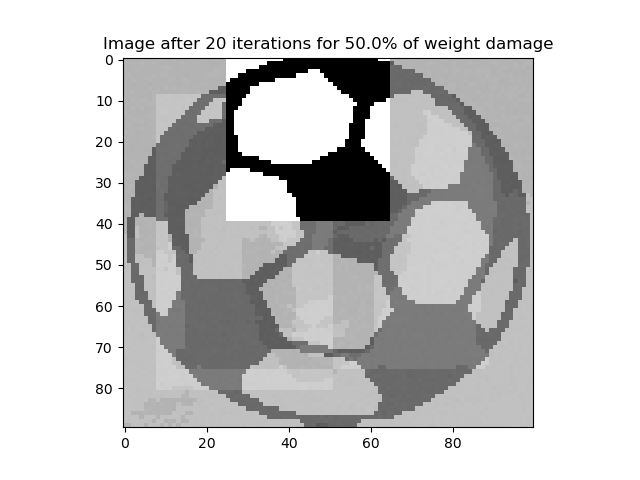
\includegraphics[width=\textwidth]{Q42}
    \captionof{figure}{At 20 iterations}
    \label{fig:Q1_1}
\end{minipage}
\hfill
\begin{minipage}{0.45\linewidth}
    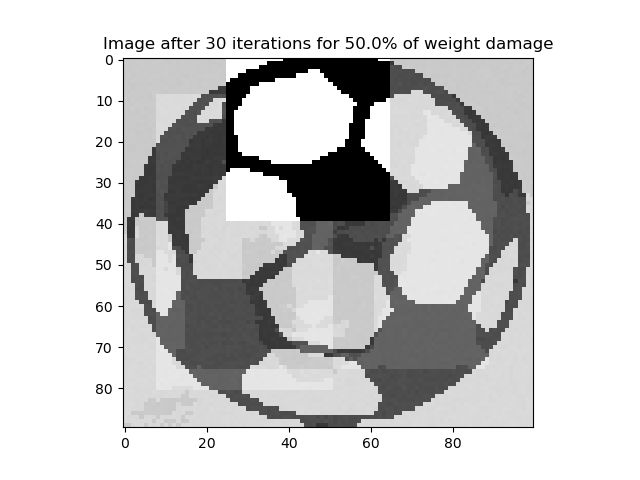
\includegraphics[width=\textwidth]{Q43}
    \captionof{figure}{At 30 iterations}
    \label{fig:Q1_2}
\end{minipage}
\vspace{1.5 em}

\begin{minipage}{0.45\linewidth}
    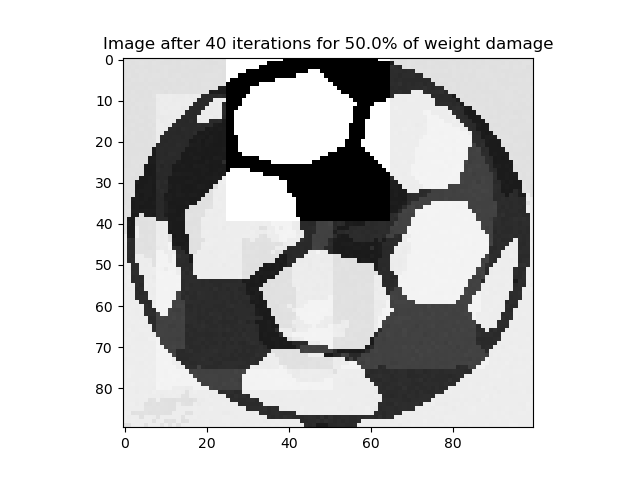
\includegraphics[width=\textwidth]{Q44}
    \captionof{figure}{At 40 iterations}
    \label{fig:Q1_1}
\end{minipage}
\hfill
\begin{minipage}{0.45\linewidth}
    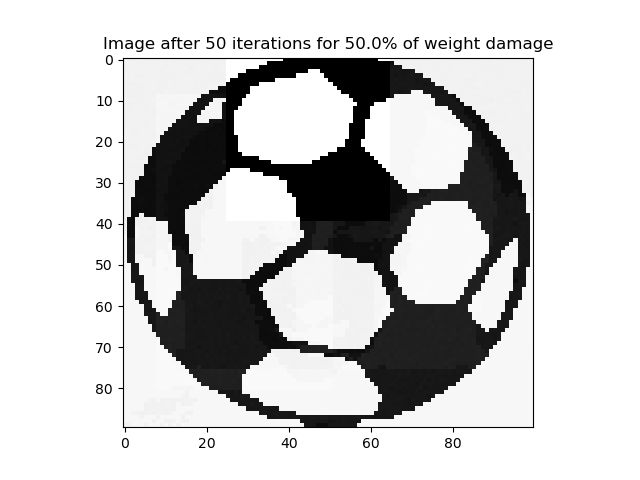
\includegraphics[width=\textwidth]{Q45}
    \captionof{figure}{At 50 iterations}
    \label{fig:Q1_2}
\end{minipage}
\vspace{1.5 em}

\begin{minipage}{0.45\linewidth}
    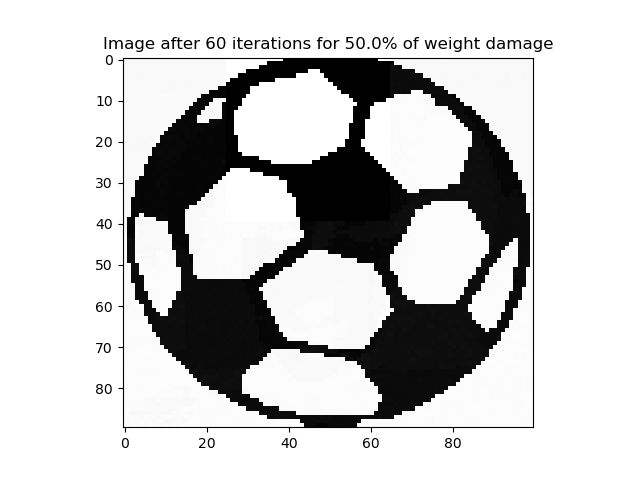
\includegraphics[width=\textwidth]{Q46}
    \captionof{figure}{At 60 iterations}
    \label{fig:Q1_1}
\end{minipage}
\hfill
\begin{minipage}{0.45\linewidth}
    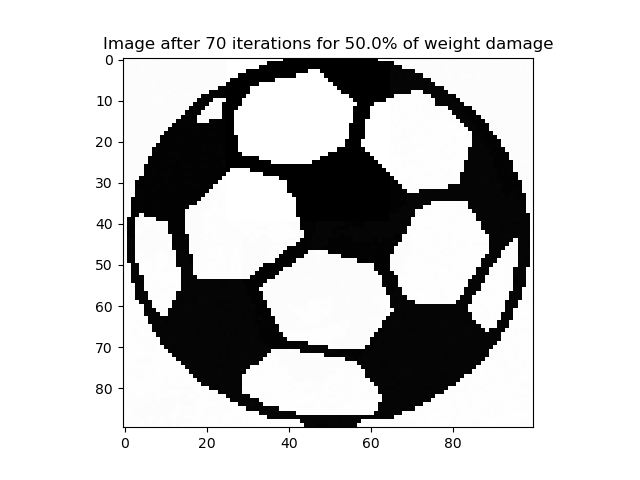
\includegraphics[width=\textwidth]{Q47}
    \captionof{figure}{At 70 iterations}
    \label{fig:Q1_2}
\end{minipage}
\vspace{1.5 em}

\begin{minipage}{0.45\linewidth}
    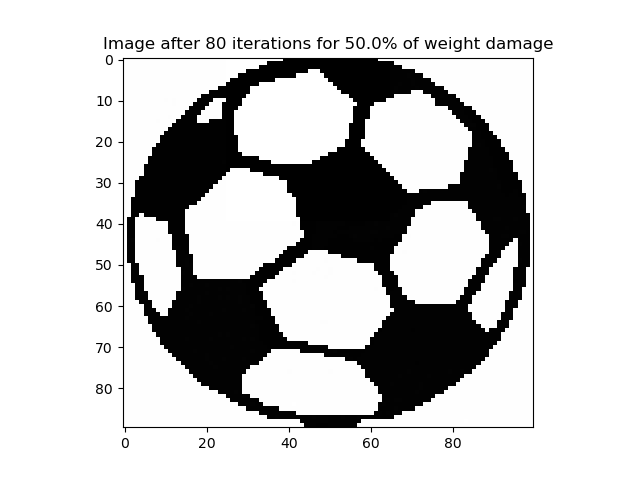
\includegraphics[width=\textwidth]{Q48}
    \captionof{figure}{At 80 iterations}
    \label{fig:Q1_1}
\end{minipage}
\hfill
\begin{minipage}{0.45\linewidth}
    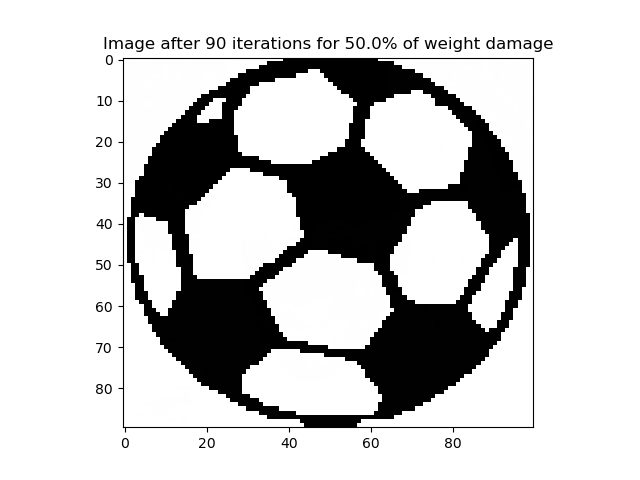
\includegraphics[width=\textwidth]{Q49}
    \captionof{figure}{At 90 iterations}
    \label{fig:Q1_2}
\end{minipage}
\vspace{1.5 em}
\end{center}

\subsection{Root mean squared error}

\begin{center}
\begin{minipage}{0.7\linewidth}
    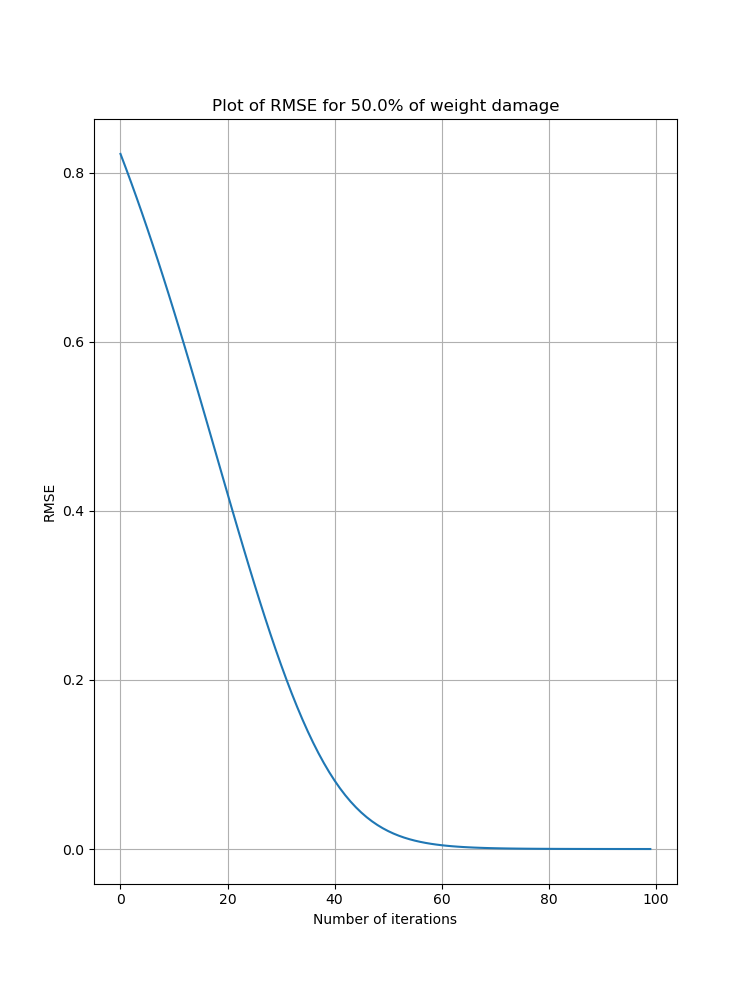
\includegraphics[width=\textwidth]{rmse_Q4}
    \captionof{figure}{RMSE for 100 iteration at 50\% weightage}
    \label{fig:Q1_3}
\end{minipage}
\end{center}

\section{80\% Weightage for Ball}

\subsection{Simulation}
\begin{center}
\begin{minipage}{0.45\linewidth}
    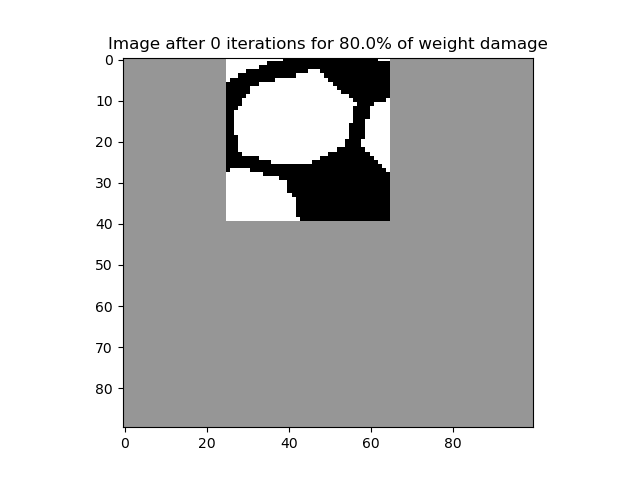
\includegraphics[width=\textwidth]{Q50}
    \captionof{figure}{At 0 iterations}
    \label{fig:Q1_1}
\end{minipage}
\hfill
\begin{minipage}{0.45\linewidth}
    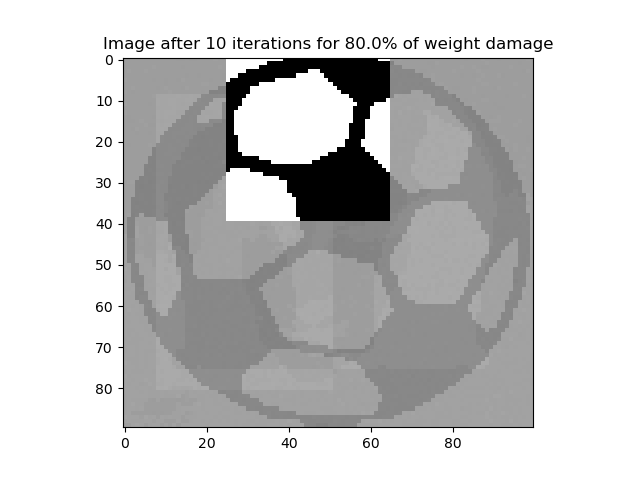
\includegraphics[width=\textwidth]{Q51}
    \captionof{figure}{At 10 iterations}
    \label{fig:Q1_2}
\end{minipage}
\vspace{1.5 em}

\begin{minipage}{0.45\linewidth}
    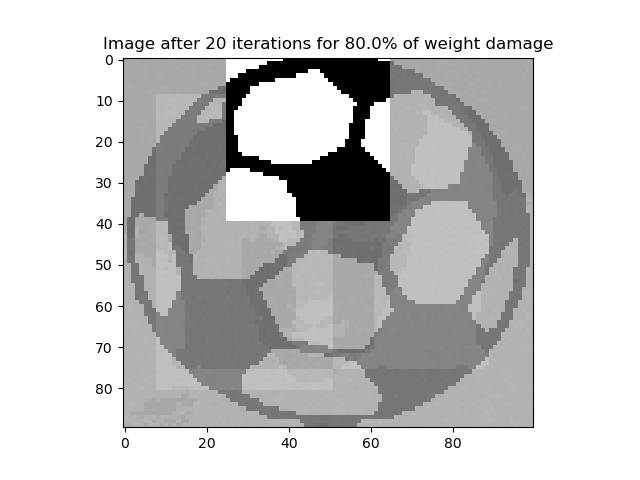
\includegraphics[width=\textwidth]{Q52}
    \captionof{figure}{At 20 iterations}
    \label{fig:Q1_1}
\end{minipage}
\hfill
\begin{minipage}{0.45\linewidth}
    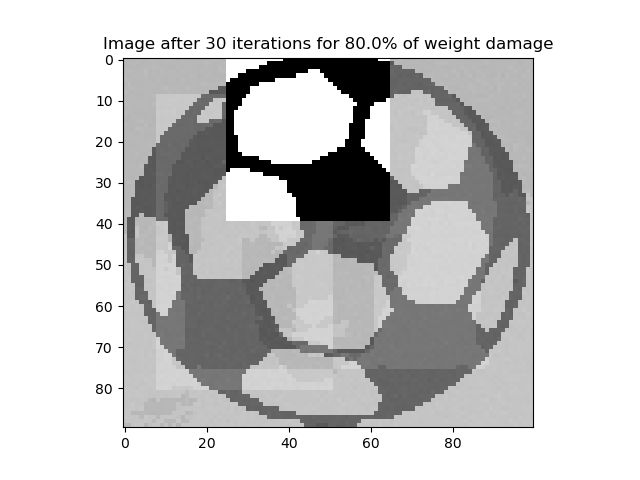
\includegraphics[width=\textwidth]{Q53}
    \captionof{figure}{At 30 iterations}
    \label{fig:Q1_2}
\end{minipage}
\vspace{1.5 em}

\begin{minipage}{0.45\linewidth}
    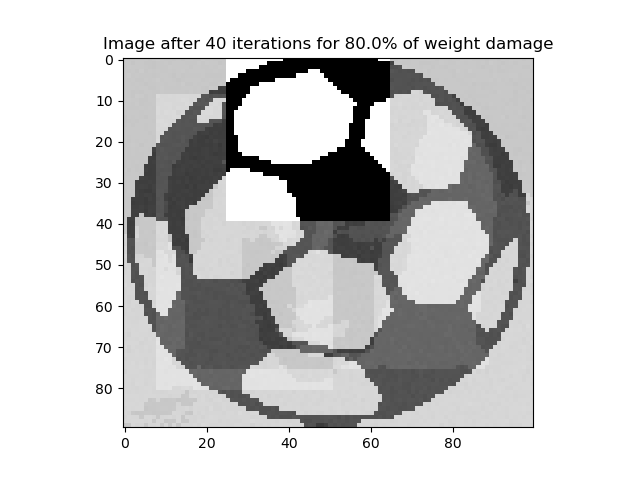
\includegraphics[width=\textwidth]{Q54}
    \captionof{figure}{At 40 iterations}
    \label{fig:Q1_1}
\end{minipage}
\hfill
\begin{minipage}{0.45\linewidth}
    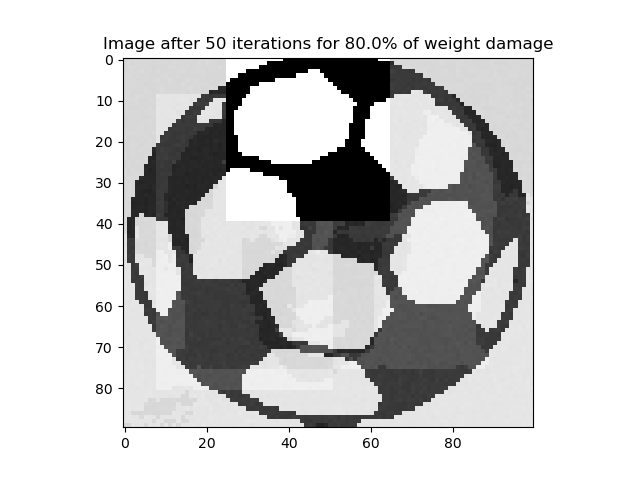
\includegraphics[width=\textwidth]{Q55}
    \captionof{figure}{At 50 iterations}
    \label{fig:Q1_2}
\end{minipage}
\vspace{1.5 em}

\begin{minipage}{0.45\linewidth}
    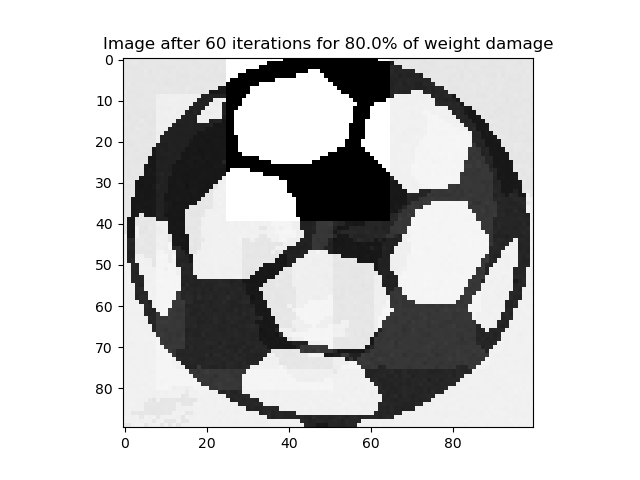
\includegraphics[width=\textwidth]{Q56}
    \captionof{figure}{At 60 iterations}
    \label{fig:Q1_1}
\end{minipage}
\hfill
\begin{minipage}{0.45\linewidth}
    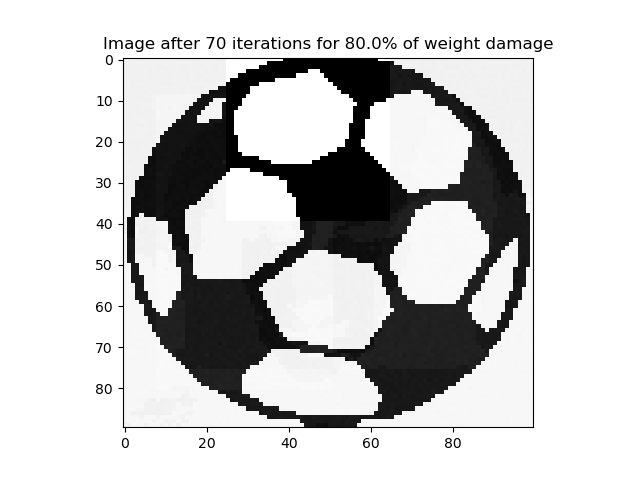
\includegraphics[width=\textwidth]{Q57}
    \captionof{figure}{At 70 iterations}
    \label{fig:Q1_2}
\end{minipage}
\vspace{1.5 em}

\begin{minipage}{0.45\linewidth}
    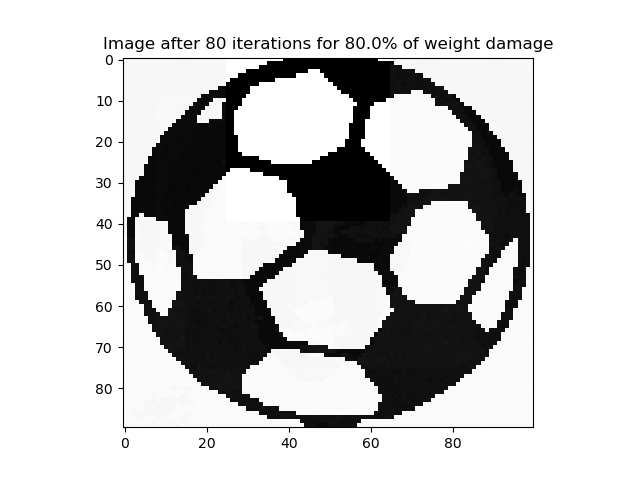
\includegraphics[width=\textwidth]{Q58}
    \captionof{figure}{At 80 iterations}
    \label{fig:Q1_1}
\end{minipage}
\hfill
\begin{minipage}{0.45\linewidth}
    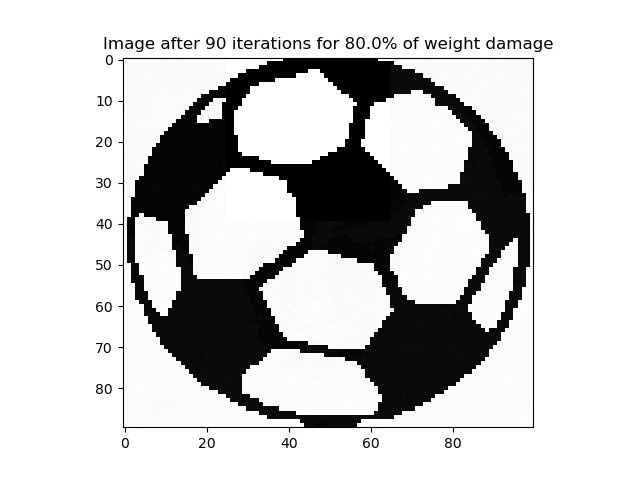
\includegraphics[width=\textwidth]{Q59}
    \captionof{figure}{At 90 iterations}
    \label{fig:Q1_2}
\end{minipage}
\vspace{1.5 em}
\end{center}

\subsection{Root mean squared error}

\begin{center}
\begin{minipage}{0.7\linewidth}
    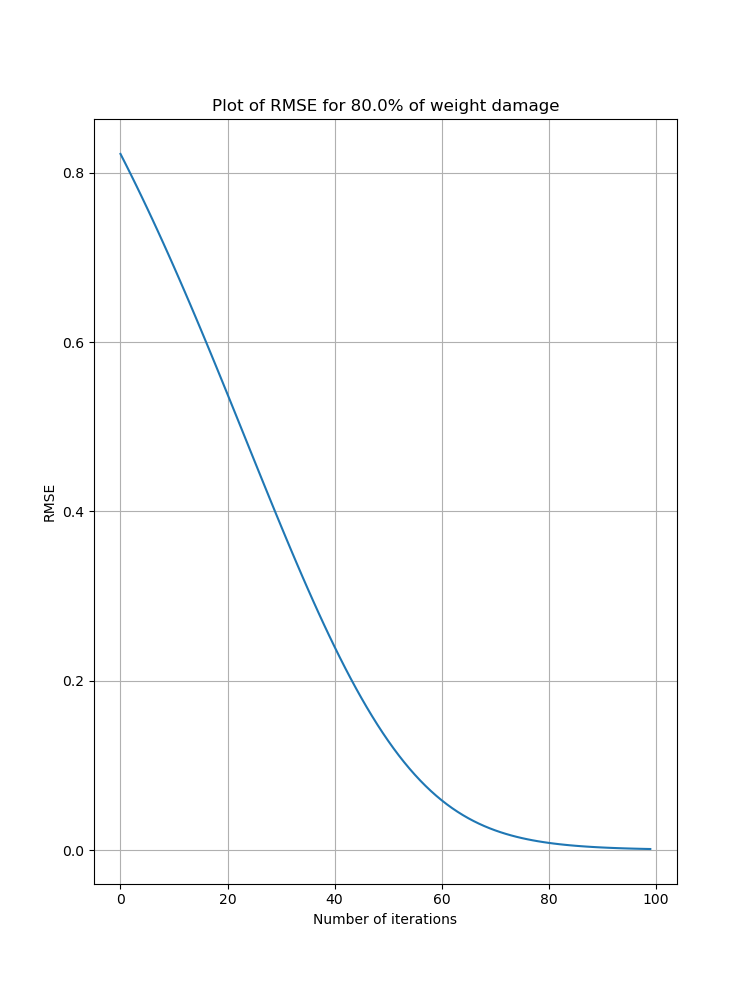
\includegraphics[width=\textwidth]{rmse_Q5}
    \captionof{figure}{RMSE for 100 iteration at 50\% weightage}
    \label{fig:Q1_3}
\end{minipage}
\end{center}

\section{0\% Weightage for Cat image}

\subsection{Simulation}
\begin{center}
\begin{minipage}{0.45\linewidth}
    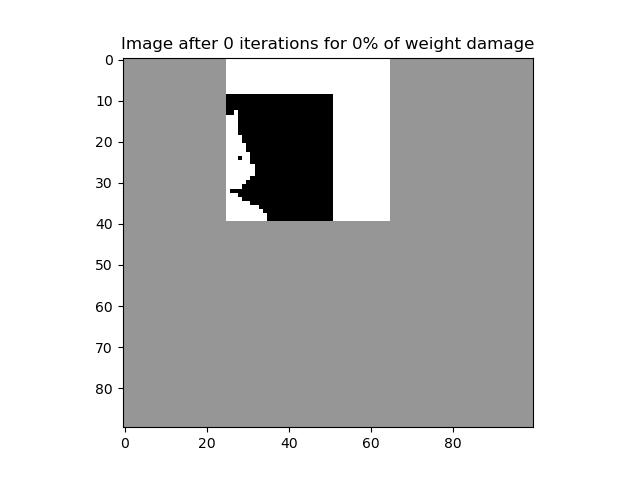
\includegraphics[width=\textwidth]{catQ20}
    \captionof{figure}{At 0 iterations}
    \label{fig:Q1_1}
\end{minipage}
\hfill
\begin{minipage}{0.45\linewidth}
    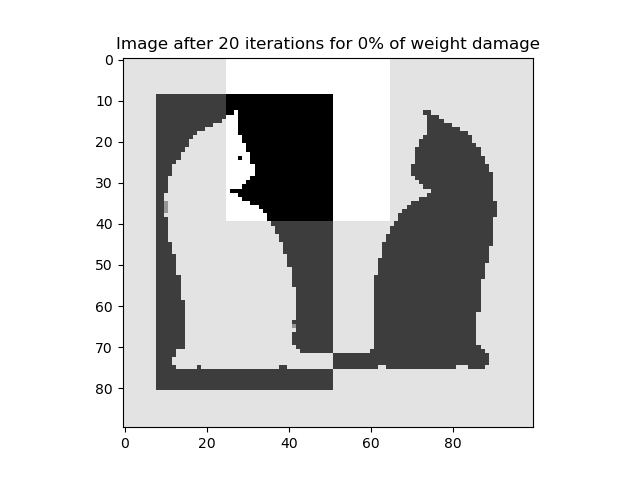
\includegraphics[width=\textwidth]{catQ22}
    \captionof{figure}{At 20 iterations}
    \label{fig:Q1_2}
\end{minipage}
\vspace{1.5 em}

\begin{minipage}{0.45\linewidth}
    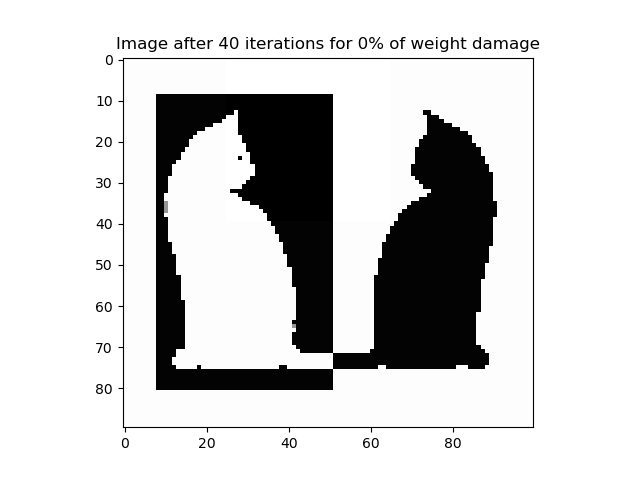
\includegraphics[width=\textwidth]{catQ24}
    \captionof{figure}{At 40 iterations}
    \label{fig:Q1_2}
\end{minipage}
\vspace{1.5 em}
\end{center}

\subsection{Root mean squared error}

\begin{center}
\begin{minipage}{0.5\linewidth}
    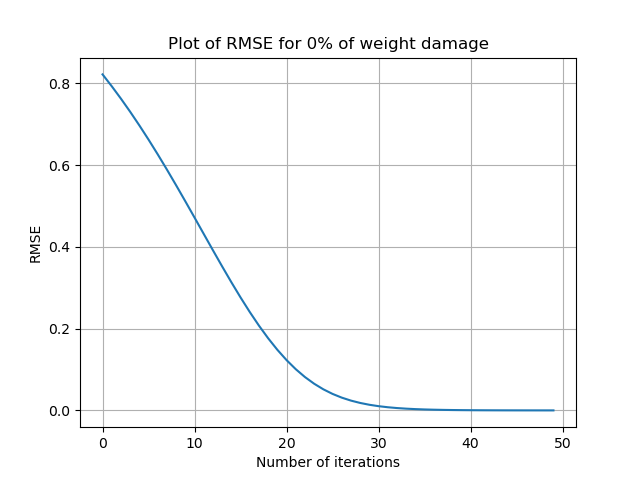
\includegraphics[width=\textwidth]{catrmse4}
    \captionof{figure}{RMSE for 100 iteration at 0\% weightage}
    \label{fig:Q1_3}
\end{minipage}
\end{center}

\section{25\% Weightage for Cat image}

\subsection{Simulation}
\begin{center}
\begin{minipage}{0.45\linewidth}
    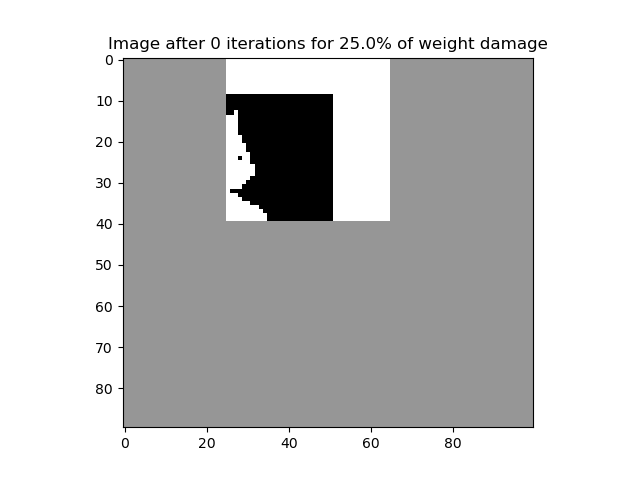
\includegraphics[width=\textwidth]{catQ30}
    \captionof{figure}{At 0 iterations}
    \label{fig:Q1_1}
\end{minipage}
\hfill
\begin{minipage}{0.45\linewidth}
    \includegraphics[width=\textwidth]{catQ34}
    \captionof{figure}{At 40 iterations}
    \label{fig:Q1_2}
\end{minipage}
\vspace{1.5 em}

\begin{minipage}{0.45\linewidth}
    \includegraphics[width=\textwidth]{catQ39}
    \captionof{figure}{At 90 iterations}
    \label{fig:Q1_2}
\end{minipage}
\vspace{1.5 em}
\end{center}

\subsection{Root mean squared error}

\begin{center}
\begin{minipage}{0.5\linewidth}
    \includegraphics[width=\textwidth]{catrmse4}
    \captionof{figure}{RMSE for 100 iteration at 25\% weightage}
    \label{fig:Q1_3}
\end{minipage}
\end{center}


\section{50\% Weightage for Cat image}
\subsection{Simulation}
\begin{center}
\begin{minipage}{0.45\linewidth}
    \includegraphics[width=\textwidth]{catQ40}
    \captionof{figure}{At 0 iterations}
    \label{fig:Q1_1}
\end{minipage}
\hfill
\begin{minipage}{0.45\linewidth}
    \includegraphics[width=\textwidth]{catQ44}
    \captionof{figure}{At 40 iterations}
    \label{fig:Q1_2}
\end{minipage}
\vspace{1.5 em}

\begin{minipage}{0.45\linewidth}
    \includegraphics[width=\textwidth]{catQ49}
    \captionof{figure}{At 90 iterations}
    \label{fig:Q1_2}
\end{minipage}
\vspace{1.5 em}
\end{center}

\subsection{Root mean squared error}

\begin{center}
\begin{minipage}{0.5\linewidth}
    \includegraphics[width=\textwidth]{catrmse4}
    \captionof{figure}{RMSE for 100 iteration at 50\% weightage}
    \label{fig:Q1_3}
\end{minipage}
\end{center}


\section{80\% Weightage for Cat image}
\subsection{Simulation}
\begin{center}
\begin{minipage}{0.45\linewidth}
    \includegraphics[width=\textwidth]{catQ50}
    \captionof{figure}{At 0 iterations}
    \label{fig:Q1_1}
\end{minipage}
\hfill
\begin{minipage}{0.45\linewidth}
    \includegraphics[width=\textwidth]{catQ54}
    \captionof{figure}{At 40 iterations}
    \label{fig:Q1_2}
\end{minipage}
\vspace{1.5 em}

\begin{minipage}{0.45\linewidth}
    \includegraphics[width=\textwidth]{catQ59}
    \captionof{figure}{At 90 iterations}
    \label{fig:Q1_2}
\end{minipage}
\vspace{1.5 em}
\end{center}

\subsection{Root mean squared error}

\begin{center}
\begin{minipage}{0.5\linewidth}
    \includegraphics[width=\textwidth]{catrmse4}
    \captionof{figure}{RMSE for 100 iteration at 80\% weightage}
    \label{fig:Q1_3}
\end{minipage}
\end{center}

\section{0\% Weightage for Mona Lisa image}

\subsection{Simulation}
\begin{center}
\begin{minipage}{0.45\linewidth}
    \includegraphics[width=\textwidth]{monaQ20}
    \captionof{figure}{At 0 iterations}
    \label{fig:Q1_1}
\end{minipage}
\hfill
\begin{minipage}{0.45\linewidth}
    \includegraphics[width=\textwidth]{monaQ22}
    \captionof{figure}{At 20 iterations}
    \label{fig:Q1_2}
\end{minipage}
\vspace{1.5 em}

\begin{minipage}{0.45\linewidth}
    \includegraphics[width=\textwidth]{monaQ24}
    \captionof{figure}{At 40 iterations}
    \label{fig:Q1_2}
\end{minipage}
\vspace{1.5 em}
\end{center}

\subsection{Root mean squared error}

\begin{center}
\begin{minipage}{0.5\linewidth}
    \includegraphics[width=\textwidth]{mona_rmse_Q2}
    \captionof{figure}{RMSE for 100 iteration at 0\% weightage}
    \label{fig:Q1_3}
\end{minipage}
\end{center}

\section{25\% Weightage for Mona Lisa image}

\subsection{Simulation}
\begin{center}
\begin{minipage}{0.45\linewidth}
    \includegraphics[width=\textwidth]{monaQ30}
    \captionof{figure}{At 0 iterations}
    \label{fig:Q1_1}
\end{minipage}
\hfill
\begin{minipage}{0.45\linewidth}
    \includegraphics[width=\textwidth]{monaQ34}
    \captionof{figure}{At 40 iterations}
    \label{fig:Q1_2}
\end{minipage}
\vspace{1.5 em}

\begin{minipage}{0.45\linewidth}
    \includegraphics[width=\textwidth]{monaQ39}
    \captionof{figure}{At 90 iterations}
    \label{fig:Q1_2}
\end{minipage}
\vspace{1.5 em}
\end{center}

\subsection{Root mean squared error}

\begin{center}
\begin{minipage}{0.5\linewidth}
    \includegraphics[width=\textwidth]{mona_rmse_Q3}
    \captionof{figure}{RMSE for 100 iteration at 25\% weightage}
    \label{fig:Q1_3}
\end{minipage}
\end{center}


\section{50\% Weightage for Mona Lisa image}
\subsection{Simulation}
\begin{center}
\begin{minipage}{0.45\linewidth}
    \includegraphics[width=\textwidth]{monaQ40}
    \captionof{figure}{At 0 iterations}
    \label{fig:Q1_1}
\end{minipage}
\hfill
\begin{minipage}{0.45\linewidth}
    \includegraphics[width=\textwidth]{monaQ44}
    \captionof{figure}{At 40 iterations}
    \label{fig:Q1_2}
\end{minipage}
\vspace{1.5 em}

\begin{minipage}{0.45\linewidth}
    \includegraphics[width=\textwidth]{monaQ49}
    \captionof{figure}{At 90 iterations}
    \label{fig:Q1_2}
\end{minipage}
\vspace{1.5 em}
\end{center}

\subsection{Root mean squared error}

\begin{center}
\begin{minipage}{0.5\linewidth}
    \includegraphics[width=\textwidth]{mona_rmse_Q4}
    \captionof{figure}{RMSE for 100 iteration at 50\% weightage}
    \label{fig:Q1_3}
\end{minipage}
\end{center}


\section{80\% Weightage for Mona Lisa image}
\subsection{Simulation}
\begin{center}
\begin{minipage}{0.45\linewidth}
    \includegraphics[width=\textwidth]{monaQ50}
    \captionof{figure}{At 0 iterations}
    \label{fig:Q1_1}
\end{minipage}
\hfill
\begin{minipage}{0.45\linewidth}
    \includegraphics[width=\textwidth]{monaQ54}
    \captionof{figure}{At 40 iterations}
    \label{fig:Q1_2}
\end{minipage}
\vspace{1.5 em}

\begin{minipage}{0.45\linewidth}
    \includegraphics[width=\textwidth]{monaQ59}
    \captionof{figure}{At 90 iterations}
    \label{fig:Q1_2}
\end{minipage}
\vspace{1.5 em}
\end{center}

\subsection{Root mean squared error}

\begin{center}
\begin{minipage}{0.5\linewidth}
    \includegraphics[width=\textwidth]{mona_rmse_Q5}
    \captionof{figure}{RMSE for 100 iteration at 80\% weightage}
    \label{fig:Q1_3}
\end{minipage}
\end{center}

\section{Conclusion}

Although the images are damaged, the retrieval is good and the original images are retrieved in about 100 iterations. This shows how good the model of Hopfield network is.

\end{document}
